\documentclass{exam}
\usepackage[utf8]{inputenc}
\usepackage{pdfpages}
\usepackage{listings}
\usepackage{mathabx}
\usepackage{graphicx}
\usepackage{float}

\date{November 6, 2019}

\begin{document}

\begin{titlepage}
\title{CSC420 Assignment 3}
\author{Mengning Yang \\
Student Number: 1002437552 \\
}
\maketitle
\end{titlepage}

\begin{questions}

\question SIFT Matching
\begin{parts}
%Q1(a)
\part Feature extraction: Compute SIFT features for reference.png, test.png, and test2.png. You can use e.g. function sift() from existing pack- ages to output, for each image, a list of feature descriptors and a list of their corresponding frames. Please visualize the detected keypoints on the image. By visualize we mean: plot the image, mark the center of each keypoint, and draw either a circle or rectangle to indicate the scale of each keypoint. For clarity, please plot only 100 keypoints. Please write the visualization function yourself – a function that loops over the extracted keypoints, and displays each keypoint on the image.

\begin{lstlisting}[language=python, frame=single]
import cv2
import numpy as np
from matplotlib import pyplot as plt
import matplotlib.patches as patches
from skimage import data
from PIL import Image

if __name__ == '__main__':
    
    imgname1 = '/Users/CYANG/Desktop/CSC420A3/reference.png'
    imgname2 = '/Users/CYANG/Desktop/CSC420A3/test.png'
    imgname3 = '/Users/CYANG/Desktop/CSC420A3/test2.png'

    sift = cv2.xfeatures2d.SIFT_create()
    img = np.array(Image.open(imgname3), dtype=np.uint8)
    kp,desc = sift.detectAndCompute(img,None)

    # Create figure and axes
    fig,ax = plt.subplots(1)

    # Display the image
    ax.imshow(img)

    for i in range(100):
        # Create a Rectangle patch
        rect = patches.Rectangle(kp[i].pt,kp[i].size*10,kp[i].size*10,
        linewidth=1,edgecolor='r',facecolor='none')

        # Add the patch to the Axes
        ax.add_patch(rect)

    plt.show()

\end{lstlisting}

\begin{figure}[H]
\caption{100 keypoints extracted using SIFT on reference.png }
\centering
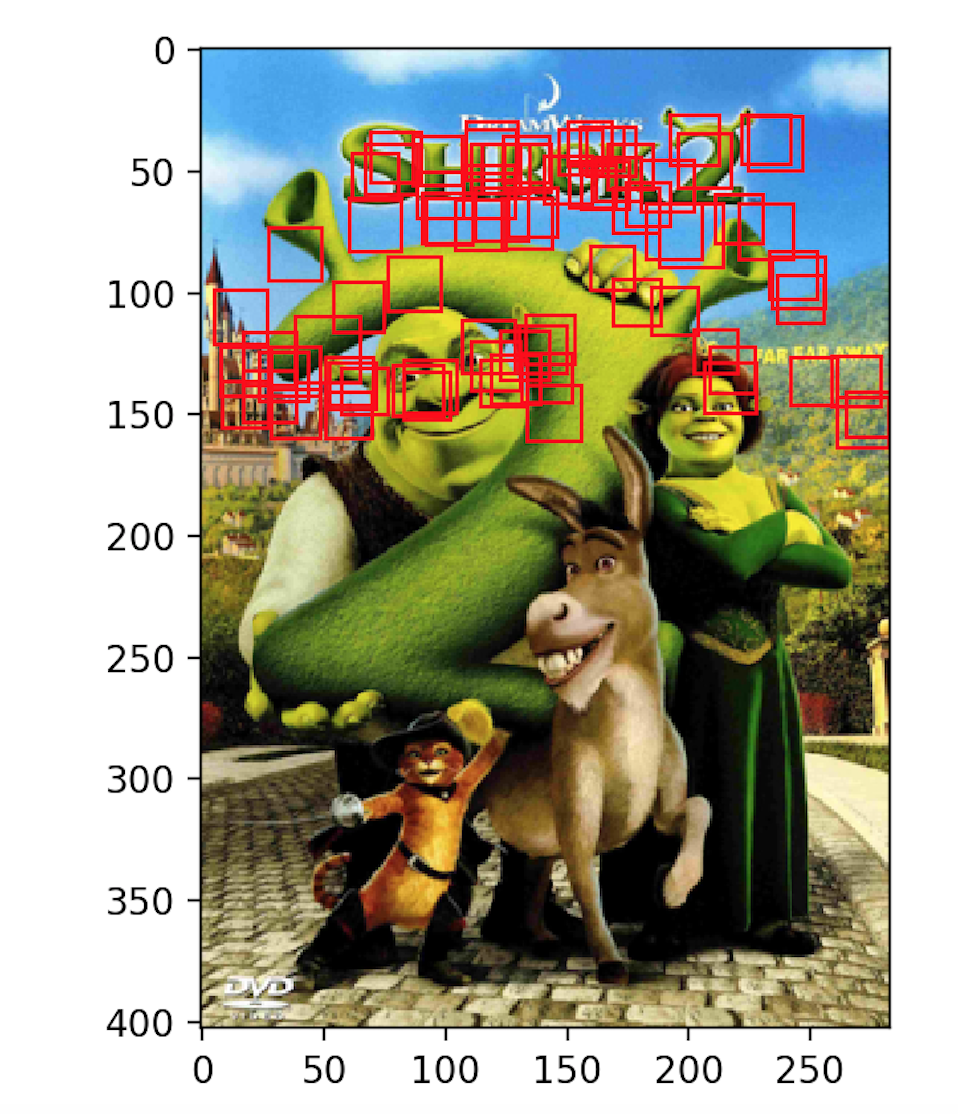
\includegraphics[width=10cm]{Q1result1.png}
\end{figure}

\begin{figure}[H]
\caption{100 keypoints extracted using SIFT on test.png }
\centering
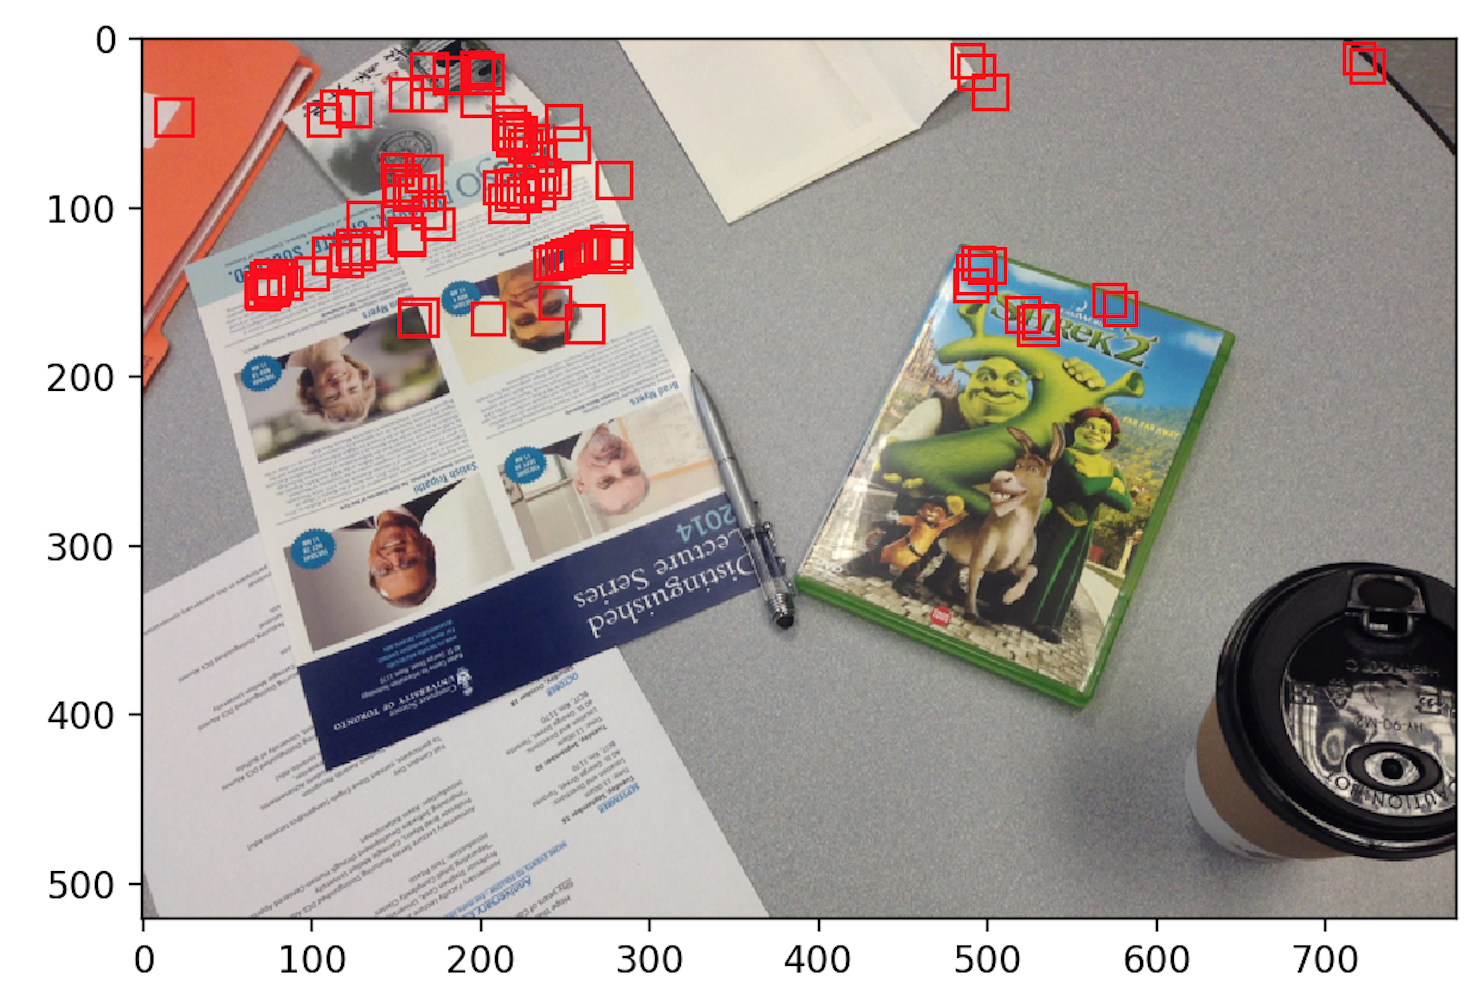
\includegraphics[width=14cm]{Q1result2.png}
\end{figure}

\begin{figure}[H]
\caption{100 keypoints extracted using SIFT on test2.png }
\centering
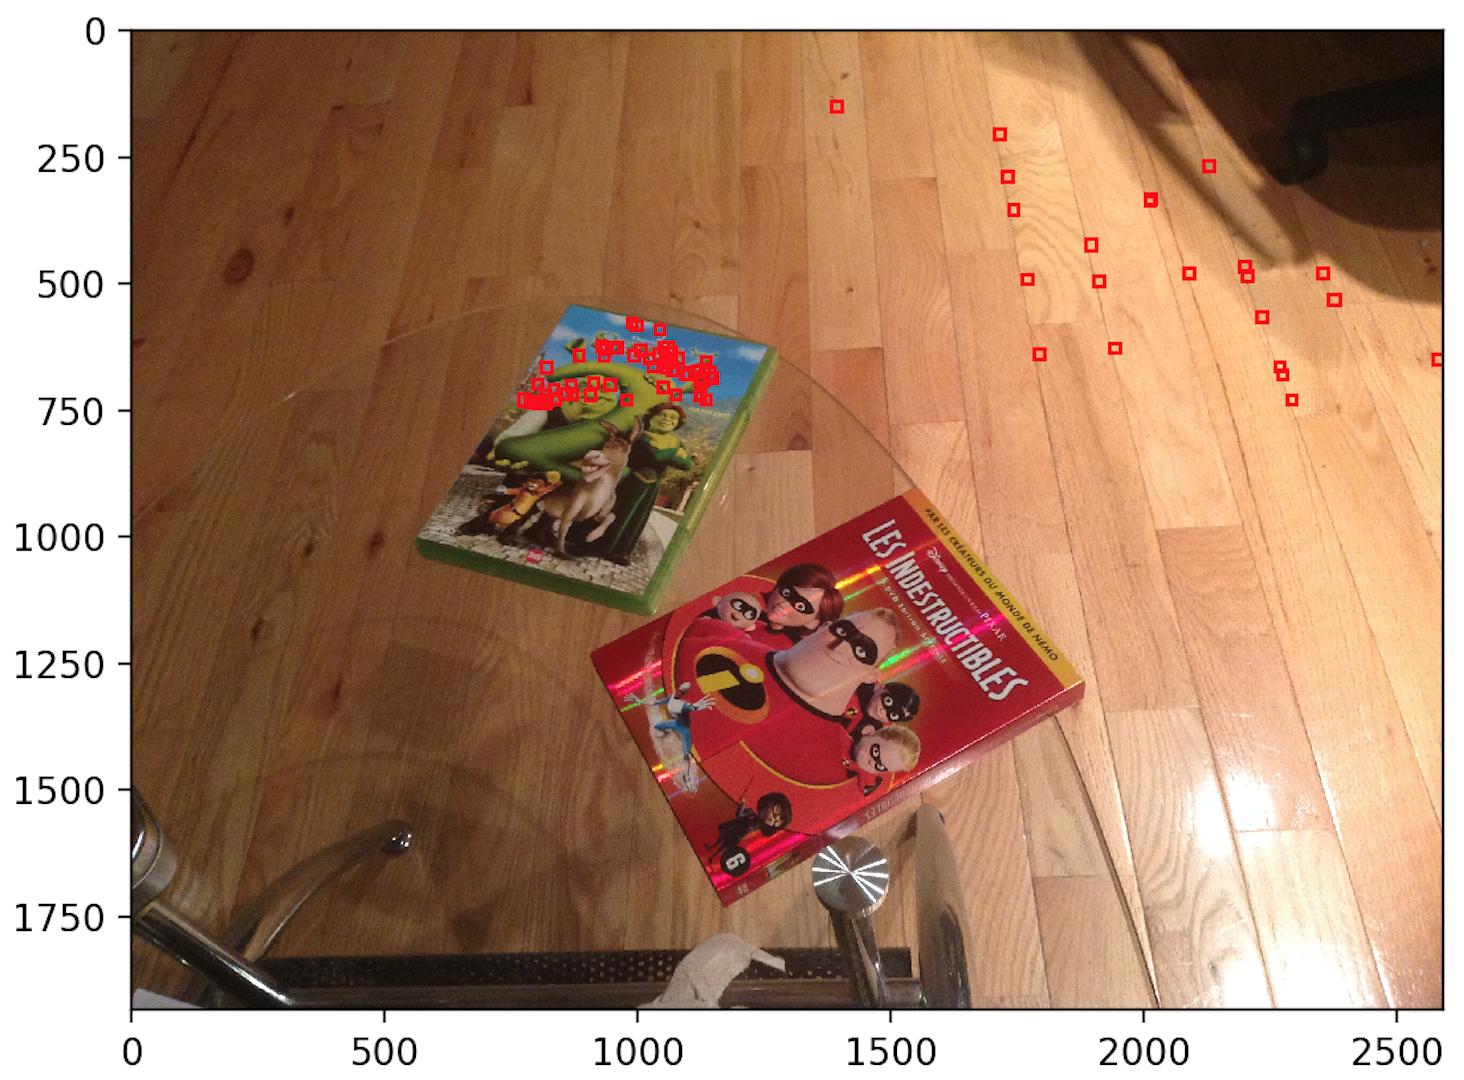
\includegraphics[width=14cm]{Q1result3.png}
\end{figure}




\newpage

%Q1(b)
\part Matching: Given the extracted features on reference.png and test.png, describe a simple matching algorithm to find the best feature matches (correspondences) for the features in reference.png and features in image test.png. How did you define “best” matches? Implement the algorithm in your favorite programming language. Visualize the top (best) 3 correspondences. Please describe what you chose as a criteria to evaluate best matches. Please do the same using the test image test2.png. Show each image and visualize each cor- respondence by indicating the feature’s position and scale in the appropriate image. Use a separate color for each correspondence.\\

Explanation of matching algorithm to find the best feature matches (correspondences) for the features in reference.png and features in image test.png.:
\begin{itemize}
\item First, find SIFT interest points in both images. And extract SIFT descriptors around each interest point. Each descriptor has location, scale, orientation and the 128 dimensional feature vector. 
\item Then, match each extracted descriptors in one image to all the descriptors found in another image by computing the euclidean distance between them. The one with shortest distance is the best match. To illustrate, if $f_{1}$ is a feature vector in the first image, and $f_{1}', ..., f_{k}'$ are the $k$-feature vectors in the second image, we compute $||f_{1} - f_{1}'||, ||f_{1} - f_{2}'||, ..., ||f_{1} - f_{k}'||$. 
\item To avoid ambiguous matches, we find the closest and second closest match. Because sometimes the best match is not really the best match, it has the shortest distance with our target maybe because it is too noisy.
\item So, we select the best match by computing the ratio between the closest and second closest match. $\phi_{i} = \frac{||f_{i} - f_{i}'*||}{||f_{i} - f_{i}'**||}$ where $f_{i}'*$ is the first closest match and $f_{i}'**$ is the second closest match. 
\item If our first match is too close to the second match, then it is an ambiguous match, and we don't want to use it to match our images. If the second match is far away from the first match, then it is a good match.
\item A common ratio used is 0.8 to prevent from getting too many false positives or too many false negatives. 
\item So, in my algorithm I only take the good matches.
\end{itemize}

\begin{lstlisting}[language=python, frame=single]
import cv2
import numpy as np
from matplotlib import pyplot as plt
import matplotlib.patches as patches
from skimage import data
from PIL import Image
from scipy import spatial

def match_sift_descriptors(left, right):
    """
    Returns a 2D array of form [[i, j, distance]], where
        i - index of a vector in left
        j - index of the closest matching vector in right
        distance - integer distance between vectors i, j
    Results are sorted by the distance of the vector pairs.
    """  
    # [i, j]-th is euclidean distance between left[i], right[j]
    euc_dists = spatial.distance.cdist(left, right, 'euclidean')
    
    # [i, j]-th is the index of the j-th closest right-vector to left[i]
    sort_inds = np.argsort(euc_dists, axis=1)
    
    # top 2 matches are represented by first and second columns of above
    closest, closest2 = sort_inds[:, 0], sort_inds[:, 1]
    
    # Compute distance ratios between (left, first closest right) 
    #vs. (left, second closest left)
    left_inds = np.arange(left.shape[0])
    dist_ratios =
    euc_dists[left_inds, closest] / euc_dists[left_inds, closest2]
    
    # Suppress where distance ratio is above some threshold
    suppressed = dist_ratios * (dist_ratios < 0.8)

    # Get indices where suppression didn't happen
    left_inds = np.nonzero(suppressed)[0]
    right_inds = closest[left_inds]
    
    # Pair the above indices together, determine distance of pair
    pairs = np.stack((left_inds, right_inds)).transpose()
    pair_dists = euc_dists[pairs[:, 0], pairs[:, 1]]
    
    sorted_dist_inds = np.argsort(pair_dists)
    sorted_pairs = pairs[sorted_dist_inds]
    sorted_dists =
    pair_dists[sorted_dist_inds].reshape((sorted_pairs.shape[0], 1))
    
    return np.hstack((sorted_pairs, sorted_dists)).astype(int)


def draw_keypoints(img1,kp1,img2,kp2,matches):
    '''
    kp1 is of type 'KeyPoint' and it contains attibutes like
    coordinates and scale of a key point.

    matches are list of list of the form [[i, j, distance]], where
        i - index of a vector in left
        j - index of the closest matching vector in right
    '''
    #for img1
    fig,ax = plt.subplots(1)
    ax.imshow(img1)

    color_list = ['r','g','b']
    for i in range(3):
        rect = patches.Rectangle(kp1[matches[i][0]].pt,
        (kp1[matches[i][0]].size)*10,(kp1[matches[i][0]].size)*10,
        linewidth=1,edgecolor=color_list[i],facecolor='none')
        ax.add_patch(rect)
    plt.show()

    #for img2
    fig,ax = plt.subplots(1)
    ax.imshow(img2)
    for i in range(3):
        rect = patches.Rectangle(kp2[matches[i][1]].pt,
        (kp2[matches[i][1]].size)*10,(kp2[matches[i][1]].size)*10,
        linewidth=1,edgecolor=color_list[i],facecolor='none')
        ax.add_patch(rect)

    plt.show()
    
    
if __name__ == '__main__':

    imgname1 = '/Users/CYANG/Desktop/CSC420A3/reference.png'
    imgname2 = '/Users/CYANG/Desktop/CSC420A3/test.png'
    imgname3 = '/Users/CYANG/Desktop/CSC420A3/test2.png'

    sift = cv2.xfeatures2d.SIFT_create()

    img1 = np.array(Image.open(imgname1), dtype=np.uint8)
    kp1,desc1 = sift.detectAndCompute(img1,None)

    img2 = np.array(Image.open(imgname3), dtype=np.uint8)
    kp2,desc2 = sift.detectAndCompute(img2,None)

    matches = match_sift_descriptors(desc1, desc2)

    draw_keypoints(img1,kp1,img2,kp2,matches)

\end{lstlisting}

\begin{figure}[H]
   \begin{minipage}{0.48\textwidth}
     \centering
     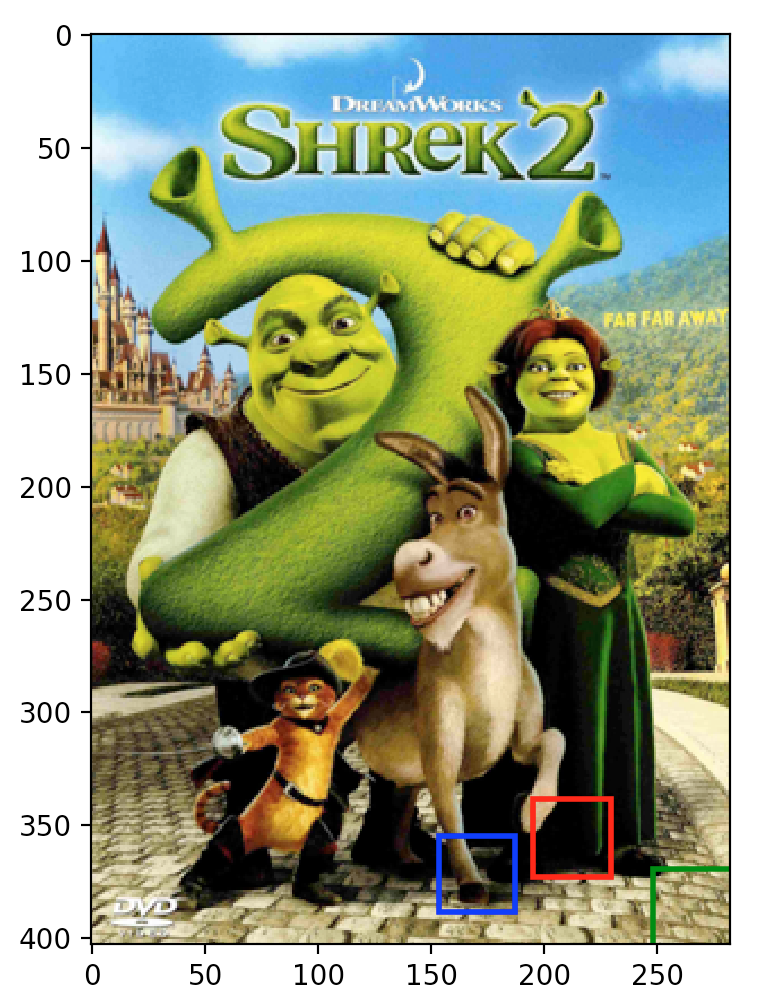
\includegraphics[width=0.8\linewidth]{Q1b1.png}
     \caption{Matching top 3 keypoints on reference.png and test.png}\label{Fig:Data1}
   \end{minipage}\hfill
   \begin{minipage}{0.48\textwidth}
     \centering
     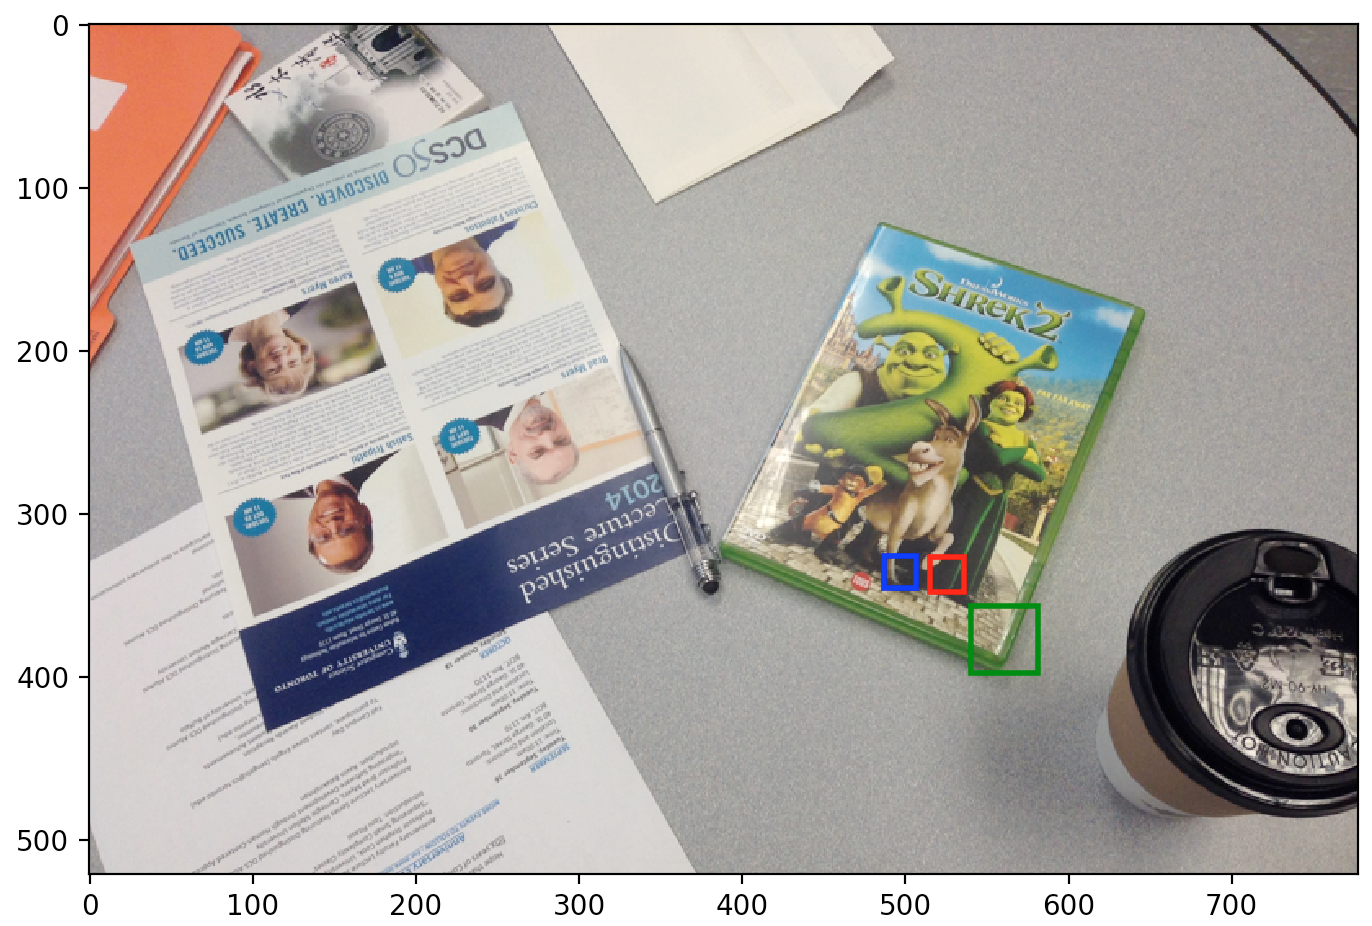
\includegraphics[width=1.3\linewidth]{Q1b2.png}
     \caption{Matching top 3 keypoints on reference.png and test.png}\label{Fig:Data2}
   \end{minipage}
\end{figure}

\newpage

\begin{figure}[H]
   \begin{minipage}{0.48\textwidth}
     \centering
     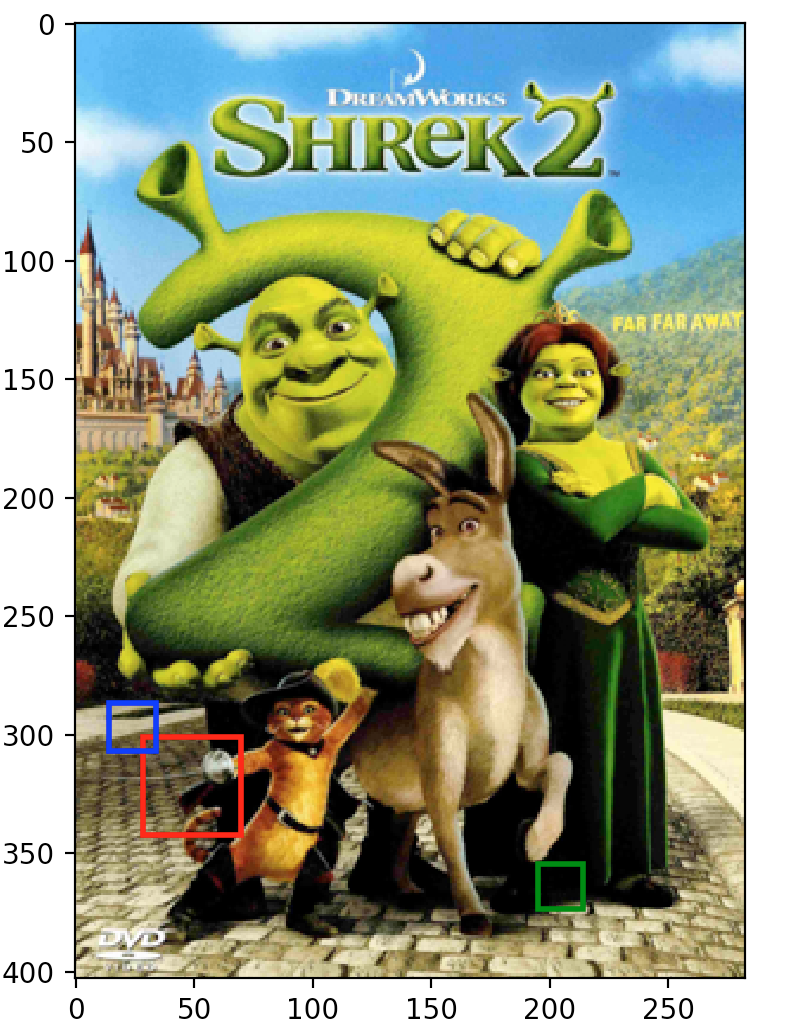
\includegraphics[width=0.8\linewidth]{Q1b3.png}
     \caption{Matching top 3 keypoints on reference.png and test2.png}\label{Fig:Data1}
   \end{minipage}\hfill
   \begin{minipage}{0.48\textwidth}
     \centering
     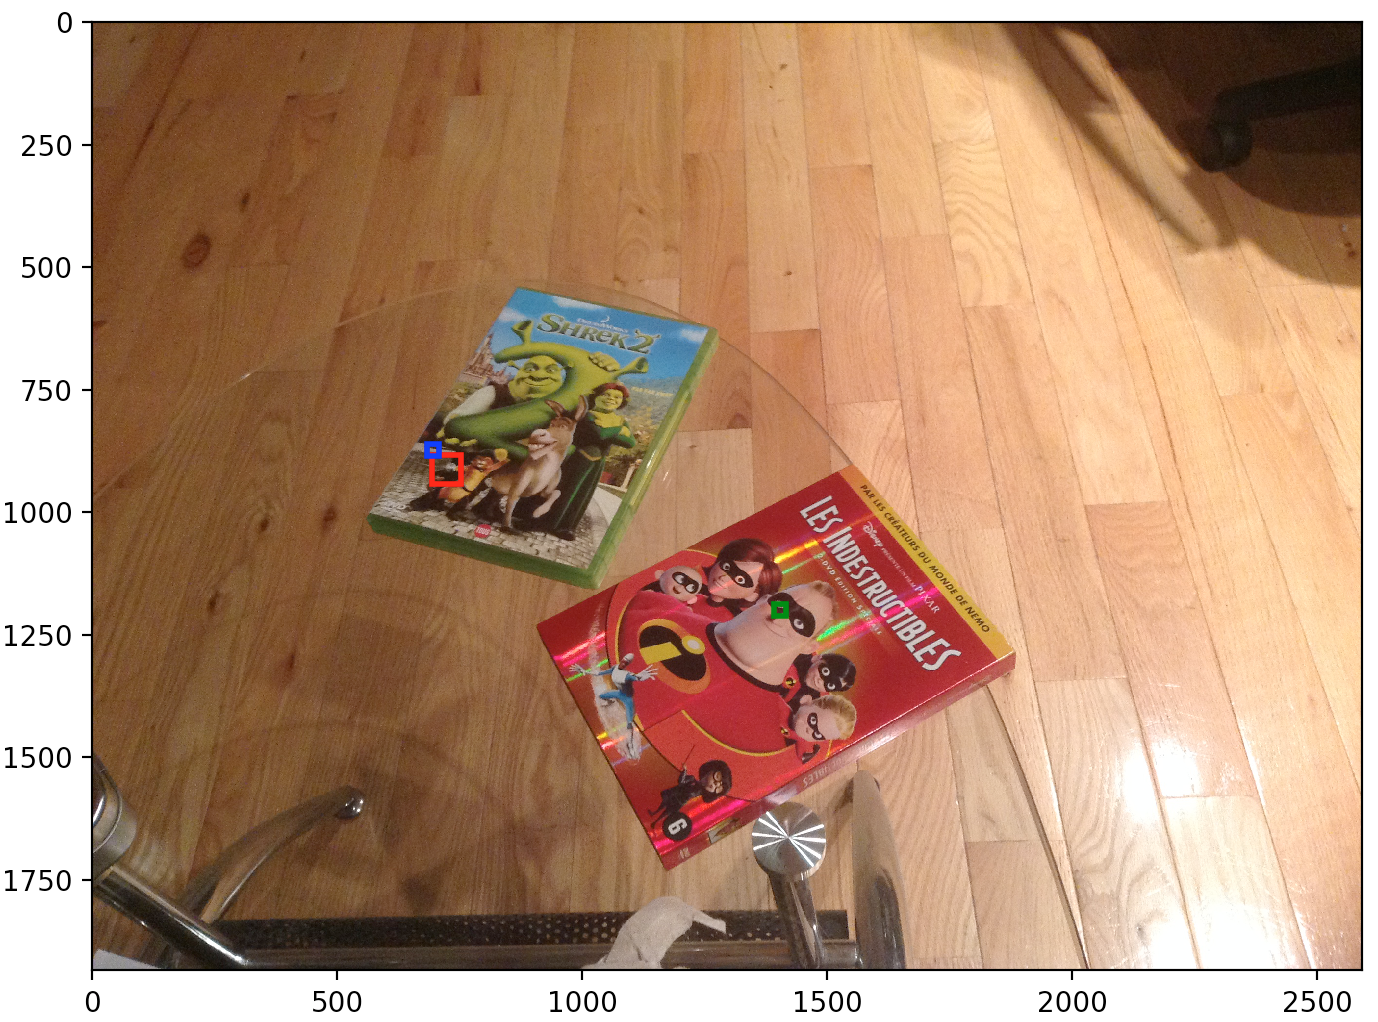
\includegraphics[width=1.3\linewidth]{Q1b4.png}
     \caption{Matching top 3 keypoints on reference.png and test2.png}\label{Fig:Data2}
   \end{minipage}
\end{figure}



%Q1(c)
\part Affine transformation: Use the top 3 correspondences from part (b) to solve for the affine transformation between the features in the two images.\\
\begin{lstlisting}[language=python, frame=single]
import cv2
import numpy as np
from matplotlib import pyplot as plot
import matplotlib.patches as patches
from skimage import data
from PIL import Image
from scipy import spatial

# Left : Source, Right : Target
def keypoints_to_coords(keypoints):
    """
    Converts keypoints into a numpy array of form [[x, y]]
    """
    return np.array([kp.pt for kp in keypoints])

def affine_left_matrix(coords):
    """
    Input: array of form [[x, y]]
    Returns a 2D array of form
    [   ...
        [x, y, 0, 0, 1, 0]
        [0, 0, x, y, 0, 1]
        ...
    ]
    """
    # Need to have 6 columns, and twice as many rows
    ret_dims = (coords.shape[0] * 2, 6)
    ret = np.empty(ret_dims, coords.dtype)
    
    # Use numpy indexing
    i = np.arange(coords.shape[0])
    
    # Even Rows: [x, y, 0, 0, 1, 0]
    ret[2*i, :2] = coords[i]
    ret[2*i, 2:] = [0, 0, 1, 0]
    
    # Odd Rows: [0, 0, x, y, 0, 1]
    ret[2*i + 1, :2] = [0, 0]
    ret[2*i + 1, 2:4] = coords[i]
    ret[2*i + 1, 4:] = [0, 1]
    
    return ret
    
def affine_right_matrix(coords):
    """
    Returns a 2D array of form 
    [
        [x]
        [y]
        ...
    ]
    """   
    # Return array needs to be twice as long
    ret = np.empty(coords.shape[0] * 2, dtype = coords.dtype)
    
    # Use numpy indexing
    i = np.arange(coords.shape[0])
    
    # Even Rows = x
    ret[2*i] = coords[i, 0]
    
    # Odd Rows = y 
    ret[2*i + 1] = coords[i, 1]
    
    return ret
    
def solve_affine_transform(left_kp_coords, right_kp_coords, k):
    
    assert k >= 3
    
    top_left, top_right = left_kp_coords[:k], right_kp_coords[:k]
    assert top_left.shape == top_right.shape
    
    # Using equation from lecture 8B: PA = P' -> A = P_inv * P'
    P = affine_left_matrix(top_left)
    P_prime = affine_right_matrix(top_right)
    
    # Compute inverse using moore-penrose pseudo inverse
    P_inv = np.linalg.pinv(P)
    
    # Approximation of affine transformation vector (a, b, c, d, e, f)
    (a, b, c, d, e, f) = np.matmul(P_inv, P_prime).flatten()
    
    # The affine transformation matrix
    return np.array(
        [[a, b, e],
         [c, d, f]]
    )
    

def affine_transform(coords, transform_matrix):
    """
    Computes the affine transform of coords (form [[x, y]]) 
    with transform_matrix.
    """
    # Add ones onto the end of every row, then transpose the 
    #matrix (columns are [x, y, 1])
    num_pts, num_dims = coords.shape
    with_ones = np.ones((num_pts, num_dims + 1))
    with_ones[:, :-1] = coords
    with_ones = with_ones.transpose()
    
    # Array of form [[x...], [y...]]
    transformed = np.matmul(transform_matrix, with_ones)
    
    return transformed.transpose()
    

def draw_polygon(img, polygon_clockwise, color, thickness):
    """
    Draws the polygon whose corner points are specified in clockwise 
    order in polygon_clockwise (array of form [[x, y]]) 
    onto a copy of img.
    """
    ret = np.copy(img)
    
    num_corners = polygon_clockwise.shape[0]
    for i in range(num_corners):
        # Figure out which points to connect together
        left_ind,  right_ind = (i % num_corners),((i+1)%num_corners)
        left = polygon_clockwise[left_ind]
        right = polygon_clockwise[right_ind]
        
        # Draw a line between them (cv needs int tuples)
        left_tup = tuple(left.astype(int))
        right_tup = tuple(right.astype(int))
        cv2.line(ret, left_tup, right_tup, color, thickness)
        
    return ret

def visualize_affine_transform(polygon_clockwise,img,transform_matrix):
    """
    Visualizes the affine transformation of transform_matrix by drawing 
    a quadrilateral (corner points specified by quadr, an array of form
    [[x, y]], clockwise order) onto a copy of right_img.
    """
    # Transform the given polygon's corner points into new space
    new_poly = affine_transform(polygon_clockwise, transform_matrix)
    
    # Return the polygon drawn on the image
    return draw_polygon(img, new_poly, (0, 255, 0), 3)
    

# Shows an image, and saves it if a filename is given
def display_image(img, file_name=None):
    
    flt_img = img.astype(float)
    img_max, img_min = np.max(flt_img), np.min(flt_img)
    
    norm_img = 
    (((flt_img - img_min)/(img_max - img_min)) * 255).astype(np.uint8)
    
    if len(img.shape) == 2:
        plot.imshow(norm_img, cmap='gray')
    elif (len(img.shape) == 3):
        plot.imshow(cv2.cvtColor(norm_img, cv2.COLOR_BGR2RGB))
    plot.show()
    
    if file_name:
        cv2.imwrite(file_name, norm_img)
        
if __name__ == '__main__':

    imgname1 = '/Users/CYANG/Desktop/CSC420A3/reference.png'
    imgname2 = '/Users/CYANG/Desktop/CSC420A3/test.png'
    imgname3 = '/Users/CYANG/Desktop/CSC420A3/test2.png'

    sift = cv2.xfeatures2d.SIFT_create()

    img1 = cv2.imread(imgname1)
    kp1,desc1 = sift.detectAndCompute(img1,None)

    img2 = cv2.imread(imgname3)
    kp2,desc2 = sift.detectAndCompute(img2,None)

    matches = match_sift_descriptors(desc1, desc2)

    cover_kp_coords = keypoints_to_coords(kp1)[matches[:, 0]]
    find_cover_kp_coords = keypoints_to_coords(kp2)[matches[:, 1]]

    # Determine four corners of the book (clockwise order)
    cover_h, cover_w = img1.shape[:2]
    cover_quadr = np.array([
        [0, 0], [cover_w, 0],
        [cover_w, cover_h], [0, cover_h]
    ])

    #use top 3 matches to do affine transformation
    matrix=solve_affine_transform(cover_kp_coords,find_cover_kp_coords,3)
    
    visualized = visualize_affine_transform(cover_quadr, img2, matrix)
    display_image(visualized,"output")
\end{lstlisting}


%Q1(d)
\part Visualize the affine transformation. Do this visualization by taking the four corners of the reference image, transforming them via the computed affine transformation to the points in the second image, and plotting those transformed points. Please also plot the edges between the points to indicate the parallelogram. \\

See code in Question 1 part (c).\\

\begin{figure}[H]
\caption{showing affine transformation in test.png}
\centering
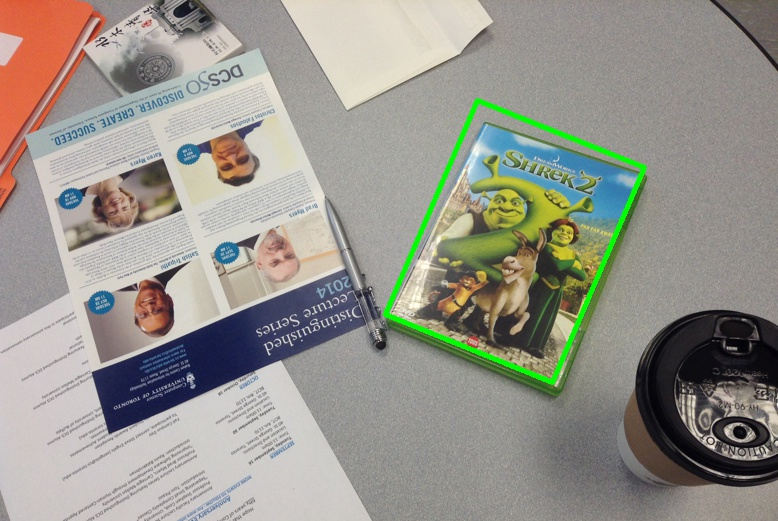
\includegraphics[width=11cm]{output.jpg}
\end{figure}

\begin{figure}[H]
\caption{showing affine transformation in test2.png}
\centering
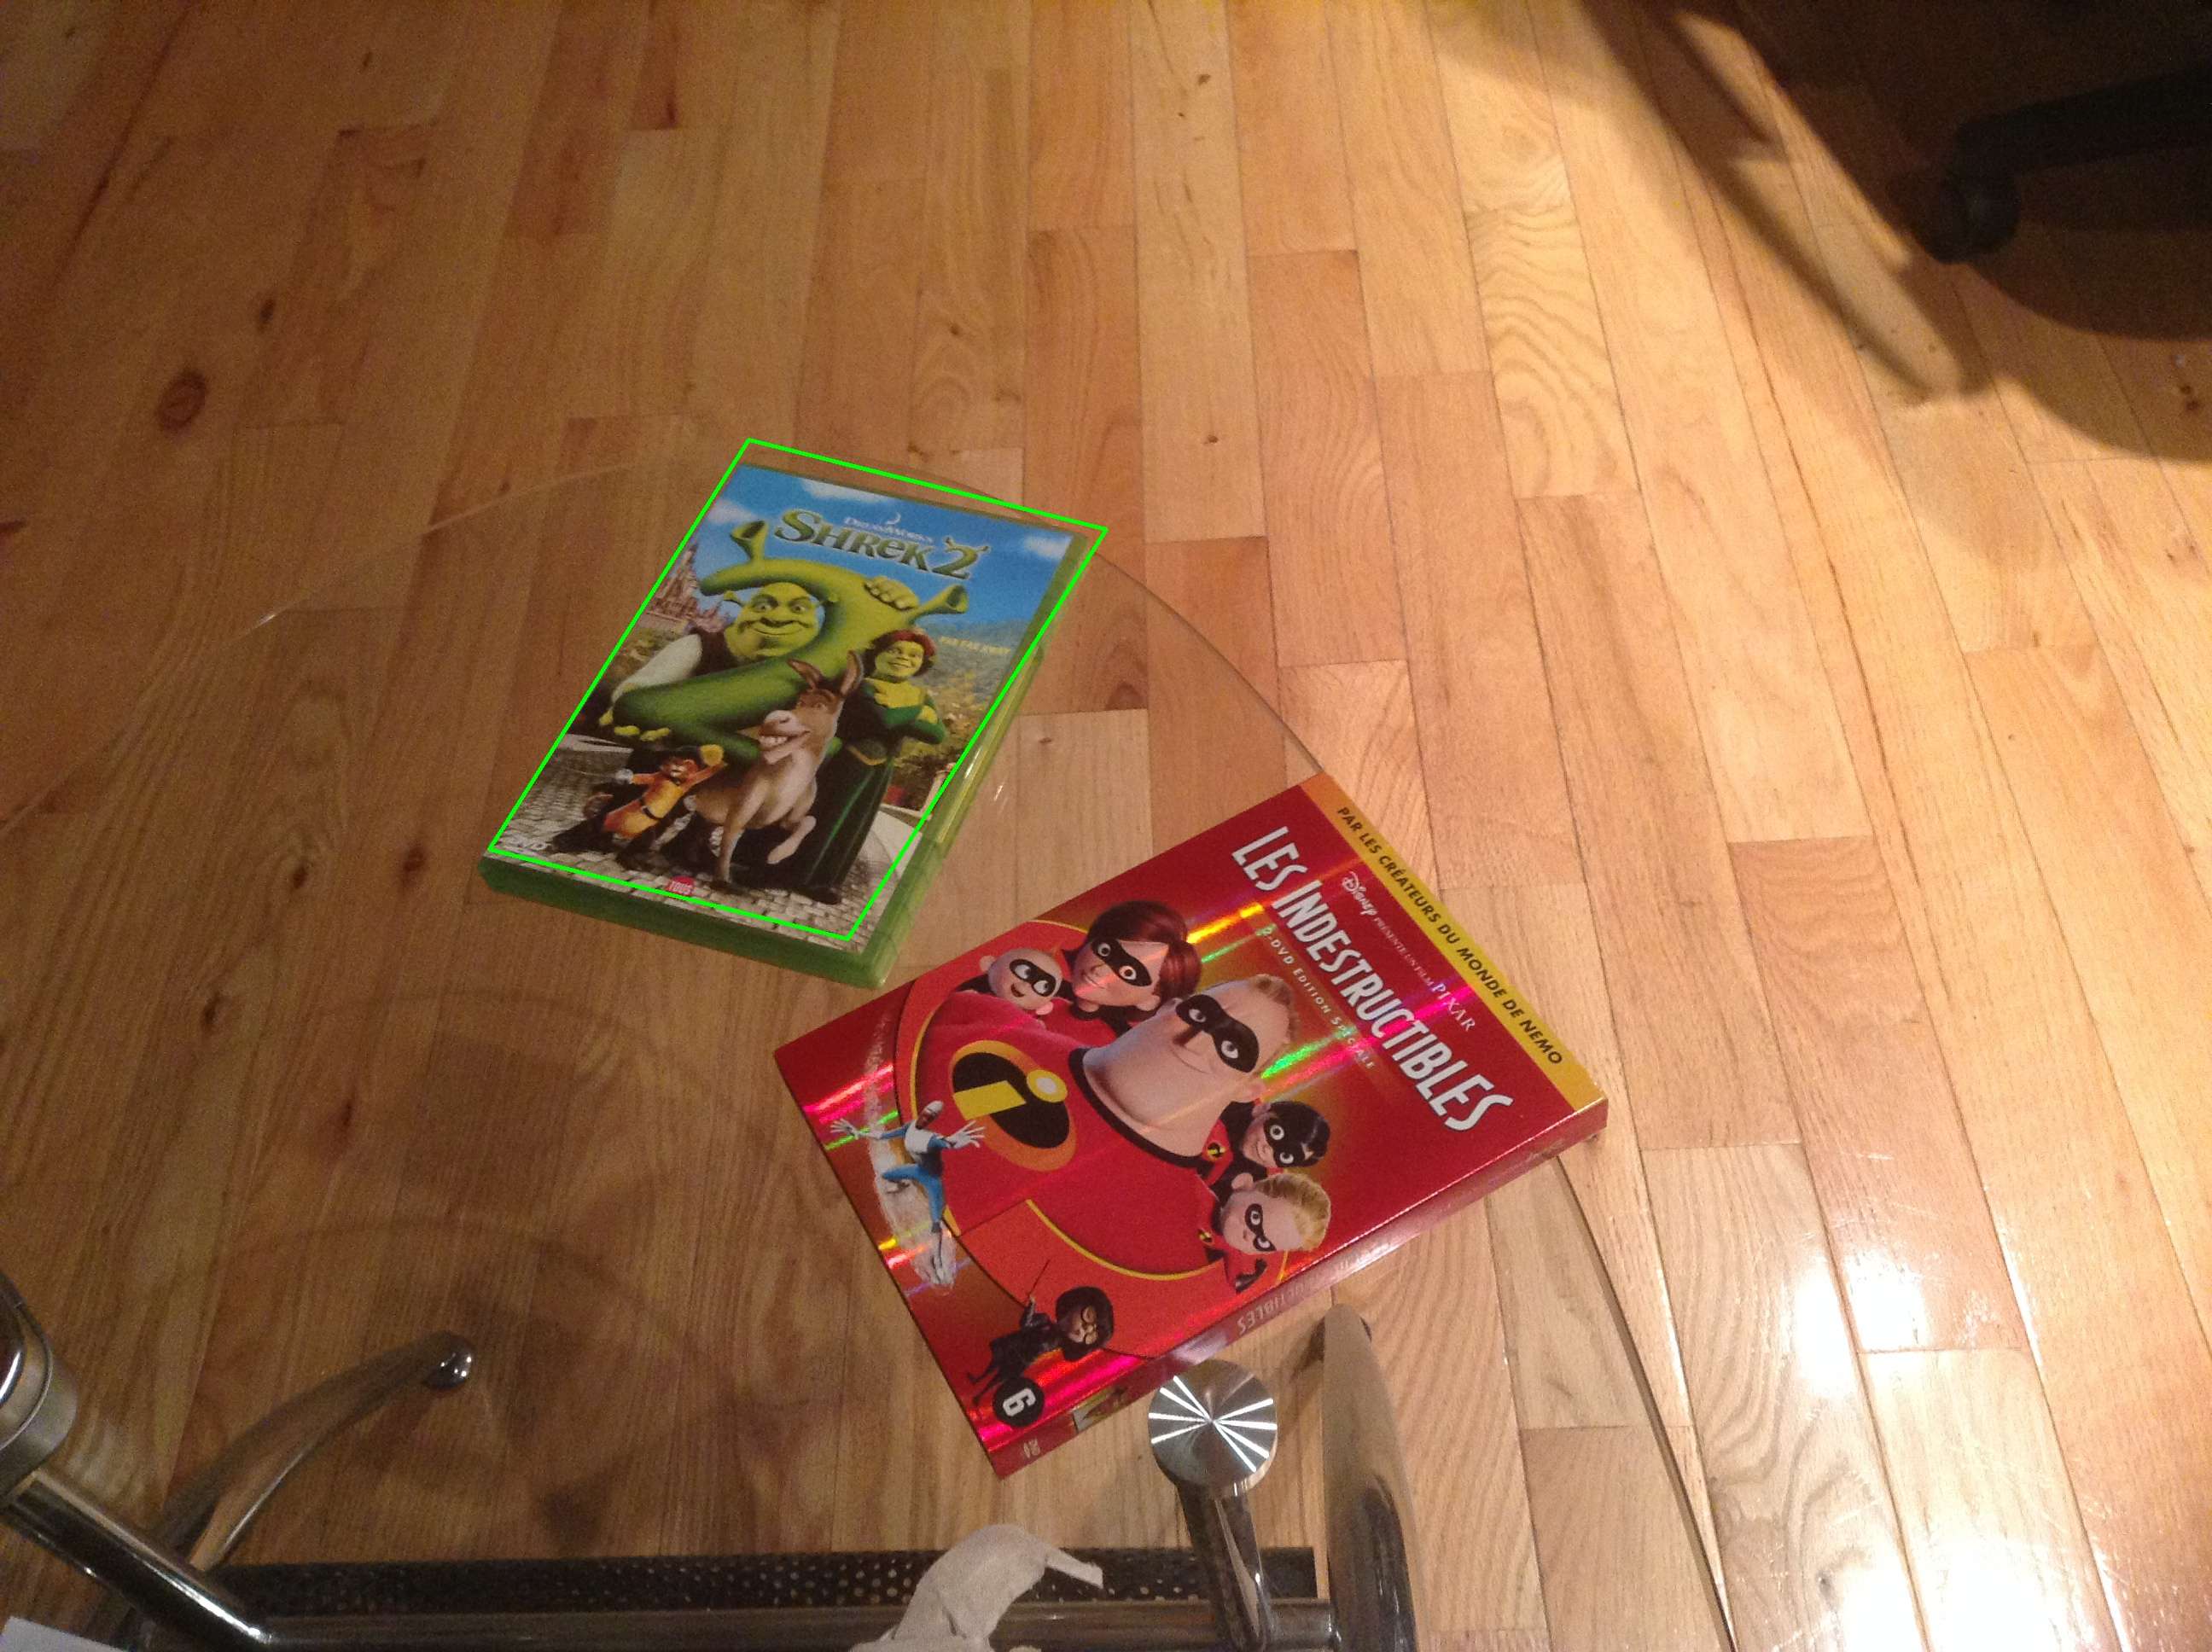
\includegraphics[width=11cm]{output2.jpg}
\end{figure}

\end{parts}\\


\question In this exercise, you are asked to take a photo. In particular, please take a planar item/object for which you know the real-world width and height (in cm), for example a piece of paper or a dollar bill. Tape the item on the door. Take a picture of the door such that all four corners of the door are visible on the photo. Take this picture in an oblique view, ie, the door is not a perfect rectangle but rather a quadrilateral in the photo. Estimate the width and height of the door (in cm) from the picture.\\

\begin{figure}[H]
\caption{photo of a door and a planar object}
\centering
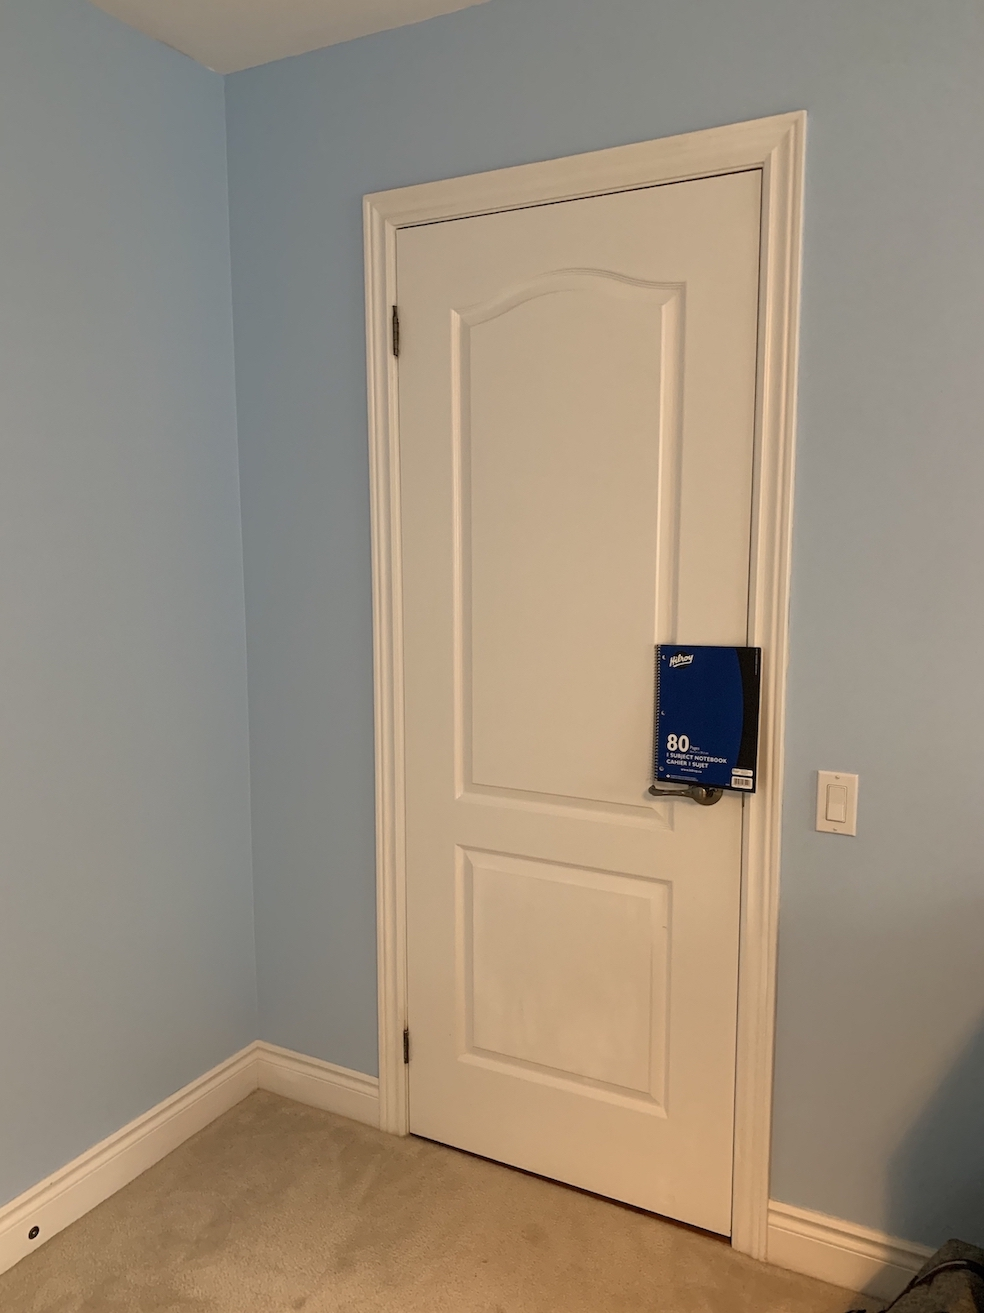
\includegraphics[width=7cm]{door.jpeg}
\end{figure}

Output:\\
Width\\
Estimate:86.32 cm\\

Height\\
Estimate:215.94 cm\\

\begin{lstlisting}[language=python, frame=single]
import numpy as np
from scipy import spatial
import cv2 as cv
import math
from matplotlib import pyplot as plot

def make_match_rows(x, y, x_prime, y_prime):
    """
    Makes two rows of match matrix A
    """
    return np.array([
        [x, y, 1, 0, 0, 0, -x_prime * x, -x_prime * y, -x_prime],
        [0, 0, 0, x, y, 1, -y_prime * x, -y_prime * y, -y_prime]
    ], dtype=float)

def make_match_matrix(matches):
    """
    Given an iterable of matches, where each match has the form 
    (x, y, x_prime, y_prime),
    make the matrix A.
    """
    return np.vstack([
        make_match_rows(x, y, x_prime, y_prime) 
        for (x, y, x_prime, y_prime) in matches
    ])

def solve_homography(matches):
    """
    Given an iterable of matches, where each match has the form 
    (x, y, x_prime, y_prime),
    compute the best homography h_hat 
    (the eigenvector of A^TA with smallest eigenvalue).
    
    Transform this eigenvector into a 3x3 matrix
    """
    A = make_match_matrix(matches)
    eig_vals, eig_vecs = np.linalg.eig(A.transpose() @ A)
    
    # Get eigenvector with smallest eigenvalue
    #(vectors are arranged vertically)
    homography_vec = eig_vecs[:, np.argmin(eig_vals)]
    
    # Reshape the homography into a matrix
    return homography_vec.reshape(3, 3)


def apply_homography(homography, cartesian_coords):
    """
    Applies homography to each coordinate in cartesian_coords.
    Returns an array of form [[x, y]], where (x, y) are the 
    homography-transformed cartesian coordinates.
    """
    # Turn the cartesian coordinates into homogeneous coordinates
    #(columns are [x, y, 1])
    homo_coords = np.array([
        (*coord, 1) 
        for coord in cartesian_coords
    ], dtype=float).transpose()
    
    # Each column is now of form ([ax', ay', a])
    transformed = homography @ homo_coords
    
    # Divide out the a's
    normalized = transformed[:2, :] / transformed[2, :]
    
    return normalized.transpose()


if __name__ == '__main__':
    door_paper = cv.imread("/Users/CYANG/Desktop/CSC420A3/door.jpeg")

    # Original coordinates of paper corners (X=21.6cm, Y=28cm)
    #corrdinates are in Top Left,Top Right,Bottom Left,Bottom Right order
    paper_cm_coords = 
    np.array([(0, 0),(21.6, 0),(0, 28),(21.6, 28)], dtype=float)

    #Pixel coordinates of paper corners
    #I used cv2.imshow() to display the image
    #and it show the coordinates when you drag your mouse
    #around on the image
    paper_pixel_coords = 
    np.array([(656, 647),(759, 651),(654, 784),(755, 796),], dtype=float)

    # Solve the homography that maps pixels to cm
    pixels_to_cm = solve_homography([(*a, *b) 
    for (a, b) in zip(paper_pixel_coords, paper_cm_coords)])

    # Pixel coordinates of door corners
    door_pixel_coords = 
    np.array([(396, 232),(761, 173),(409, 1135),(730, 1239)], dtype=float)

    # Map the door pixels into cm space
    door_cm_coords = apply_homography(pixels_to_cm, door_pixel_coords)

    # Figure out the width/height of the door
    door_x, door_y = door_cm_coords.transpose()
    door_width = max(door_x) - min(door_x)
    door_height = max(door_y) - min(door_y)
    

    print("Width")
    print("Estimate:{} cm".format(round(door_width, 2)))
    print("")

    print("Height")
    print("Estimate:{} cm".format(round(door_height, 2)))

\end{lstlisting}



%Question 3
\question You are given a few photos of landscape. The goal is to take two photos, landscape 1 and landscape 2 and stitch them into one photograph. You can do this by extracting SIFT features from both photos, match them, and estimate a homography of one photo with respect to the other. Use RANSAC to find the best homography. Once you compute the homography, “stitch” the two photos together, forming a small panorama. We will give half points if you compute affine transformation instead of a homography.

\begin{lstlisting}[language=python, frame=single]
import cv2
import numpy as np
import matplotlib.pyplot as plt
import getopt
import sys
import random
import math
from scipy import spatial


#creating homographies from random correspondences using RANSAC
def ransac(corr, k, thresh):
    maxInliers = []
    finalH = None
    for i in range(k):
        #find 4 random points to calculate a homography
        corr1 = corr[random.randrange(0, len(corr))]
        corr2 = corr[random.randrange(0, len(corr))]
        randomFour = np.vstack((corr1, corr2))
        corr3 = corr[random.randrange(0, len(corr))]
        randomFour = np.vstack((randomFour, corr3))
        corr4 = corr[random.randrange(0, len(corr))]
        randomFour = np.vstack((randomFour, corr4))

        #call the homography function on those points
        #h = calculateHomography(randomFour)
        h = calculateHomography(randomFour)
        inliers = []

        for i in range(len(corr)):
            d = geometricDistance(corr[i], h)
            if d < 5:
                inliers.append(corr[i])

        if len(inliers) > len(maxInliers):
            maxInliers = inliers
            finalH = h

        if len(maxInliers) > (len(corr)*thresh):
            break
    return finalH, maxInliers



#Calculate the geometric distance between estimated points and original points
def geometricDistance(correspondence, h):

    p1 = np.transpose(np.matrix([correspondence[0].item(0), 
    correspondence[0].item(1), 1]))
    estimatep2 = np.dot(h, p1)
    estimatep2 = (1/estimatep2.item(2))*estimatep2

    p2 = np.transpose(np.matrix([correspondence[0].item(2), 
    correspondence[0].item(3), 1]))
    error = p2 - estimatep2
    return np.linalg.norm(error)

# Computers a homography from 4-correspondences
def calculateHomography(correspondences):
    #loop through correspondences and create assemble matrix
    aList = []
    for corr in correspondences:
        p1 = np.matrix([corr.item(0), corr.item(1), 1])
        p2 = np.matrix([corr.item(2), corr.item(3), 1])

        a2 = [0, 0, 0, -p2.item(2) * p1.item(0), -p2.item(2) * p1.item(1), 
        -p2.item(2) * p1.item(2),p2.item(1) * p1.item(0), 
        p2.item(1) * p1.item(1),p2.item(1) * p1.item(2)]
        
        a1 = [-p2.item(2) * p1.item(0), -p2.item(2) * p1.item(1), 
        -p2.item(2) * p1.item(2), 0, 0, 0,p2.item(0) * p1.item(0), 
        p2.item(0) * p1.item(1), p2.item(0) * p1.item(2)]
        
        aList.append(a1)
        aList.append(a2)

    matrixA = np.matrix(aList)

    #svd composition
    u, s, v = np.linalg.svd(matrixA)

    #reshape the min singular value into a 3 by 3 matrix
    h = np.reshape(v[8], (3, 3))

    #normalize and now we have h
    h = (1/h.item(8)) * h
    return h


if __name__ == '__main__':

    imgname1 = '/Users/CYANG/Desktop/CSC420A3/landscape_1.jpg'
    imgname2 = '/Users/CYANG/Desktop/CSC420A3/landscape_2.jpg'

    img1 = cv2.imread(imgname2)
    img2 = cv2.imread(imgname1)

    sift = cv2.xfeatures2d.SIFT_create()

    kp1, des1 = sift.detectAndCompute(img1,None)
    kp2, des2 = sift.detectAndCompute(img2,None)

    estimation_thresh = 0.8

    correspondenceList = []
    if img1 is not None and img2 is not None:
        kp1, desc1 = sift.detectAndCompute(img1,None)
        kp2, desc2 = sift.detectAndCompute(img2,None)
    
        #function worte in Question 1 part (b)
        matches = match_sift_descriptors(desc1, desc2)

        for match in matches:
            (x1, y1) = kp1[match[0]].pt
            (x2, y2) = kp2[match[1]].pt
            correspondenceList.append([x1, y1, x2, y2])

        corrs = np.matrix(correspondenceList)

        finalH, inliers = ransac(corrs, 1000,estimation_thresh)
        dst = cv2.warpPerspective(img1,
        finalH,(img2.shape[1] + img1.shape[1], img2.shape[0]))
        dst[0:img2.shape[0], 0:img2.shape[1]] = img2

        result = dst[:,:,::-1]
        cv2.imshow('wooooooooowwwwww',result)
        cv2.waitKey(0)


\end{lstlisting}

\begin{figure}[H]
   \begin{minipage}{0.48\textwidth}
     \centering
     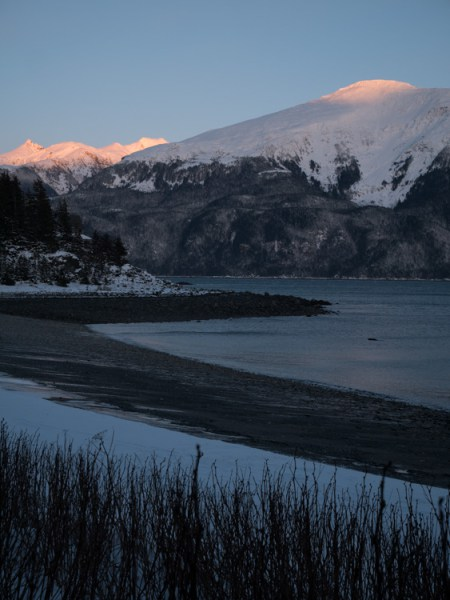
\includegraphics[width=0.8\linewidth]{landscape_1.jpg}
     \caption{Photo 1 to be stitched}\label{Fig:Data1}
   \end{minipage}\hfill
   \begin{minipage}{0.48\textwidth}
     \centering
     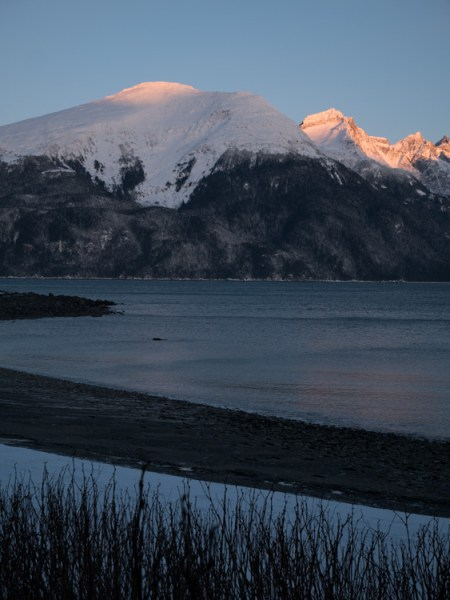
\includegraphics[width=0.8\linewidth]{landscape_2.jpg}
     \caption{Photo 2 to be stitched}\label{Fig:Data2}
   \end{minipage}
\end{figure}

\begin{figure}[H]
\caption{result of stitching photo1 and photo2 together}
\centering
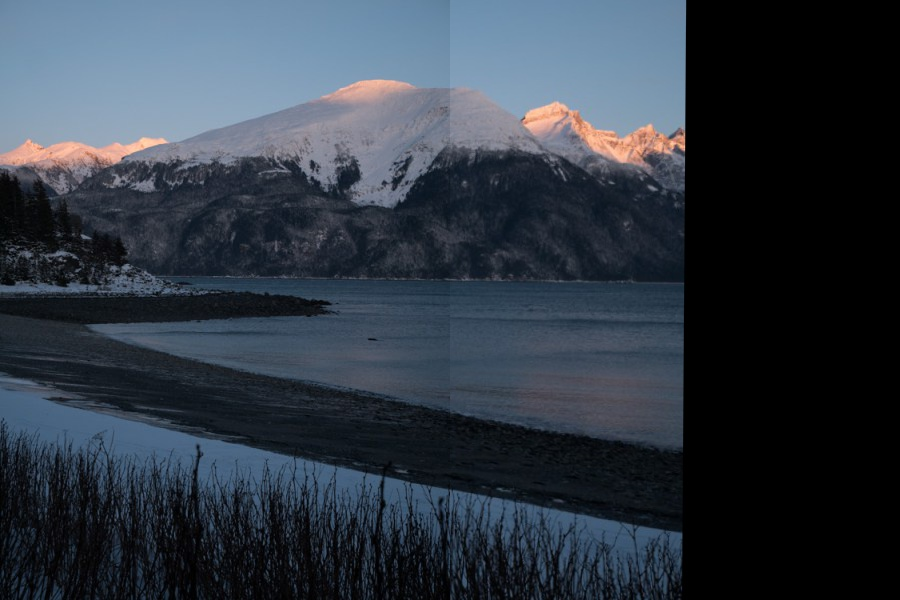
\includegraphics[width=14cm]{StitchingOutput.jpg}
\end{figure}

\end{questions}

\end{document}

